% Self-contained source. Compile twice with pdfLaTeX.
\documentclass[11pt,a4paper]{article}
\usepackage[T1]{fontenc}
\usepackage{lmodern,microtype,amsmath,amssymb,amsthm,booktabs,tabularx,array,xcolor,fancyhdr,enumitem,tikz,hyperref}
\usepackage[left=24mm,right=24mm,top=24mm,bottom=22mm,headheight=15pt]{geometry}
\definecolor{ink}{HTML}{193344}\definecolor{teal}{HTML}{08625B}
\hypersetup{colorlinks=true,linkcolor=teal,citecolor=teal,urlcolor=teal,pdftitle={Counterexamples to Lin's second distance eigenvalue bound},pdfauthor={Shaitetsu}}
\pagestyle{fancy}\fancyhf{}\renewcommand{\headrulewidth}{.3pt}
\fancyhead[L]{\sffamily\footnotesize Counterexamples to Lin's distance eigenvalue bound}
\fancyhead[R]{\sffamily\footnotesize Spectral graph theory}
\fancyfoot[L]{\sffamily\footnotesize Research manuscript\quad 16 November 2026}
\fancyfoot[R]{\sffamily\footnotesize\thepage}
\setlength{\parindent}{0pt}\setlength{\parskip}{4pt}
\setlength{\abovedisplayskip}{7pt}\setlength{\belowdisplayskip}{7pt}
\newcommand{\head}[1]{\par\medskip{\sffamily\bfseries\color{teal}#1}\par\smallskip}
\newcommand{\parthead}[2]{{\sffamily\small\bfseries\color{teal}#1}\par\vspace{2mm}{\sffamily\bfseries\color{ink}\fontsize{21}{25}\selectfont #2\par}\vspace{2mm}}
\newcommand{\one}{\mathbf1}\newcommand{\RR}{\mathbb R}\newcommand{\dd}{\,\mathrm d}
\newcommand{\hd}[1]{\textbf{#1.}}
\begin{document}
\phantomsection\pdfbookmark[0]{The problem and main results}{start}
{\sffamily\bfseries\small\color{teal} SPECTRAL GRAPH THEORY\quad /\quad RESEARCH MANUSCRIPT}\par\vspace{4mm}
{\sffamily\bfseries\color{ink}\fontsize{26}{30}\selectfont\raggedright Counterexamples to Lin's\\ second distance eigenvalue bound\par}
\vspace{2mm}
{\large Exact witnesses, positive eigenvalues of theta graphs, and their scaling limits}\par
\smallskip Shaitetsu\quad$\cdot$\quad 16 November 2026
\head{Abstract}
Huiqiu Lin asked whether the second eigenvalue of the distance matrix of every connected graph of order $n$ is at most $n/2-2$, with equality exactly for the balanced complete bipartite graph. We disprove both assertions. A graph of order 39 has second eigenvalue 18, and a graph of order 48 and diameter four attains equality. On planar bipartite graphs of maximum degree three, the largest possible $k$th distance eigenvalue has order $n^2$ for every fixed $k$. For equal-length theta graphs we compute the inertia, enclose the positive eigenvalues by an explicit cosine sequence with a two-index shift, and determine each fixed-rank limiting coefficient. All finite witnesses use ordinary unweighted graph distance.
\head{Lin's original question}
For a finite connected simple undirected graph $G$, let $D_{uv}=d_G(u,v)$, with zero diagonal. Write $\lambda_1(D)\ge\cdots\ge\lambda_n(D)$, counting multiplicity. Problem~4 in Lin's May 2018 preprint, subsequently published in 2019, asks whether
\[
 \lambda_2(D)\le \frac n2-2,\qquad
 \lambda_2(D)=\frac n2-2\ \Longleftrightarrow\ G\cong K_{n/2,n/2}.
\]
The proposed equality graph requires even $n$. Lin had proved the diameter-dependent bound $n(d-1)/2-d$, which gives the proposed inequality when $d=2$. The question reappeared as Problem~2.1 in the 2021 survey coauthored by Lin \cite{lin,survey}.
\head{What produces the quadratic growth?}
Consider several equal paths with common endpoints. Along one path the distance is $|i-j|$. Between two paths it is a constant minus the same distance after reflection. On vectors with zero sum and even reflection symmetry, summing the path contributions reverses the sign of the path distance form. Its negative is a sum of squares of partial sums. Slowly varying path profiles have large partial sums. This gives a whole subspace with large positive Rayleigh quotients. Sections below prove the count and identify the limiting spectrum. The final section records the scope of the historical evidence.
\newpage
\pdfbookmark[0]{Exact finite counterexamples}{finite}
\parthead{1\quad /\quad ORIGINAL PROBLEM}{Two exact finite witnesses}
For $q\ge3$, $m\ge1$, form $H_{q,m}$ from $2q$ disjoint independent sets $A_i,B_j$ of size $m$ and $q^2$ other vertices $e_{ij}$, with $1\le i,j\le q$. Join $e_{ij}$ to every vertex of $A_i\cup B_j$. These are all its edges. This connected bipartite graph has $n=2qm+q^2$ and diameter four. In particular, different $A$-sets lie at distance four.
\head{The short disproof}
Let $x$ take values $1$ on the $A$-sets, $-1$ on the $B$-sets, and $0$ elsewhere. From $v\in A_i$, distances to the rest of $A_i$, other $A$-sets and all $B$-sets are respectively $2,4,2$. At $e_{ij}$ the positive and negative contributions cancel by symmetry. Hence
\[
 Dx=\big(2(m-1)+4(q-1)m-2qm\big)x=\big(2(q-1)m-2\big)x.
\]
The largest eigenvalue has a strictly positive eigenvector and is simple, by Perron--Frobenius. Hence $\lambda_2\ge2(q-1)m-2$. Taking $(q,m)=(3,5)$ gives $18>35/2$. Every $m>q^2/[2(q-2)]$ gives a strict violation.
\head{The full calculation for the equality assertion}
Call each set $A_i$ or $B_j$ a cloud. A vector summing to zero inside one cloud and vanishing elsewhere has eigenvalue $-2$. On the complementary space of cloud-constant vectors write $a_i,b_j$ for their values and $C=(c_{ij})$ on the grid. Let $S_a,S_b,S_c$ denote the three totals and let $r_i,s_j$ be the row and column sums of $C$. Counting shortest paths gives
\begin{align*}
 (Dx)_{A_i}&=4m S_a-(2m+2)a_i+2m S_b+3 S_c-2r_i,\\
 (Dx)_{B_j}&=4m S_b-(2m+2)b_j+2m S_a+3 S_c-2s_j,\\
 (Dx)_{e_{ij}}&=3m(S_a+S_b)-2m(a_i+b_j)+4 S_c-2(r_i+s_j).
\end{align*}
The grid part with all margins zero has eigenvalue zero. For a zero-sum row profile $u$, set $a_i=A u_i$, $c_{ij}=C_0u_i$, $b_j=0$. On $(A,C_0)$ the matrix is
$\left(\begin{smallmatrix}-2m-2&-2q\\-2m&-2q\end{smallmatrix}\right)$,
with negative trace and positive determinant $4q$. Its eigenvalues are real by restriction of the symmetric operator. The column sector gives the same block. Every grid decomposes into its mean, row and column contrasts, and a zero-margin remainder. For constant coordinates, the antisymmetric cloud direction is the vector $x$ above. The remaining two coordinates (common cloud value, common grid value) give
\[
 Q=\begin{pmatrix}(6q-2)m-2&q(3q-2)\\2m(3q-2)&4q(q-1)\end{pmatrix}.
\]
For $(3,5)$ its eigenvalues are $51\pm\sqrt{2199}$, which straddle 18. Thus $\lambda_2=18$. For $(4,4)$ they are $67\pm\sqrt{3561}$, which straddle 22. Hence $\lambda_2=22=48/2-2$. Diameter four distinguishes this graph from $K_{24,24}$.
\newpage
\pdfbookmark[0]{Path reflection and an exact compression}{compression}
\parthead{2\quad /\quad AUXILIARY PROBLEM}{Large eigenvalues on three parallel paths}
Let $G_{q,L}$ consist of $q\ge3$ internally disjoint paths of $L=p+1\ge2$ edges with the same two endpoints. Its order is $n=qp+2$. Label internal vertices by an arm and a level $1\le i\le p$. On the same arm $d(i,j)=|i-j|$. On different arms the shorter route through an endpoint has length
\[
 \min(i+j,2L-i-j)=L-|i-(L-j)|.
\]
Traversing a whole additional arm cannot shorten either distance. In matrix notation the diagonal arm blocks are $A=(|i-j|)$ and the off-diagonal blocks are $B=LJ-AR$, where $J$ is all ones and $R$ reverses the $p$ coordinates.
\begin{center}
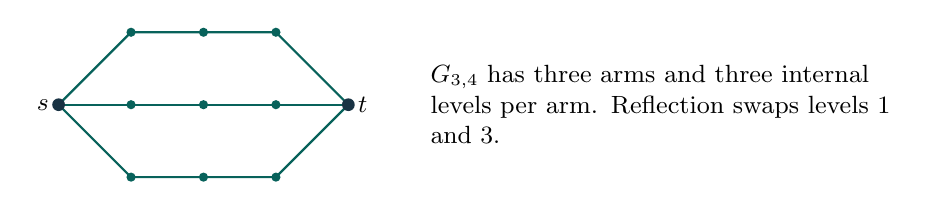
\begin{tikzpicture}[scale=.92,every node/.style={font=\small}]
\foreach \h in {-1,0,1}{
 \draw[teal,thick] (0,0)--(1,\h)--(2,\h)--(3,\h)--(4,0);
 \foreach \x in {1,2,3}{\fill[teal] (\x,\h) circle (1.8pt);}
}
\fill[ink] (0,0) circle(2.5pt);\fill[ink] (4,0) circle(2.5pt);
\node[left] at (0,0){$s$};\node[right] at (4,0){$t$};
\node[anchor=west,text width=6.0cm] at (5,0){$G_{3,4}$ has three arms and three internal levels per arm. Reflection swaps levels 1 and 3.};
\end{tikzpicture}
\end{center}
\hd{Theorem 1} Put $h=\lfloor(p-1)/2\rfloor$. For $1\le j\le h$ define
\[
 b_j=\frac{q-2}{1-\cos(2\pi j/p)}.
\]
The distance matrix has a compression with eigenvalues $b_1,\ldots,b_h$. In particular $\lambda_j(D)\ge b_j\ge(q-2)p^2/(2\pi^2j^2)$.
\head{Proof}
Set both endpoint coordinates to zero. On every arm use the same vector $f=Rf$ with $\sum_i f_i=0$. The numerator of its Rayleigh quotient is $q f^T[A+(q-1)B]f=-q(q-2) f^TAf$, and the squared norm is $q\|f\|^2$. For each cut between levels $t$ and $t+1$, summing contributions to $f^TAf$ across that cut gives twice the product of its left and right masses. Thus
\[
 -f^TAf=2\sum_{t=1}^{p-1}\Big(\sum_{i=1}^t f_i\Big)^2 .
\]
Use the orthogonal basis $f_i^{(j)}=\cos(2\pi j(i-1/2)/p)$, $1\le j\le h$. These even zero-sum vectors have norm squared $p/2$, and the space has dimension $\lceil p/2\rceil-1=h$. Their partial sums at $t$ are $\sin(2\pi jt/p)/(2\sin(\pi j/p))$. The sine profiles are orthogonal with squared norm $p/2$, by finite geometric sums. The displayed compression is therefore diagonal with the stated eigenvalues. Min--max interlacing and $1-\cos u\le u^2/2$ give the two inequalities.\hfill$\square$
\newpage
\pdfbookmark[0]{Inertia and counting}{inertia}
\parthead{3\quad /\quad FINITE SPECTRUM}{Exact inertia and the number above Lin's bound}
\hd{Theorem 2} For $q\ge3$, $p\ge1$, the numbers of positive and zero eigenvalues of $D(G_{q,p+1})$ are
\[
 n_+=\lceil p/2\rceil+1,\qquad n_0=(q-1)\lfloor p/2\rfloor .
\]
The other $qp+2-n_+-n_0$ are negative. If $3\le k\le n_+$, then $\lambda_k\le b_{k-2}$. For fixed $q$ as $p\to\infty$,
\[
 \#\{k:\lambda_k>n/2-2\}
 =\frac1\pi\sqrt{\frac{(q-2)p}{q}}+O_q(1).
\]
\head{Proof}
Arm permutations and simultaneous level reversal commute with $D$. First split off vectors with common arm profile, allowing both endpoint coordinates, from their orthogonal complement, whose endpoint coordinates vanish and whose arm values sum to zero at each level. Split each part into even and odd reflection parity. Write $K=(L/2)J-A$. This is positive definite because
\[
 K_{ij}=\tfrac12\int_0^L\operatorname{sgn}(i-u)\operatorname{sgn}(j-u)\dd u.
\]
A vanishing linear combination of these step functions has zero jump at each internal integer, forcing all coefficients to vanish.
\begin{itemize}[leftmargin=1.5em,nosep]
\item On common even profiles $f$, put $S=\sum f_i$ and let $a$ be the common endpoint coordinate. The quadratic form is
\[
 2L(a+qS/2)^2+q(q-2) f^T Kf .
\]
Indeed, endpoint pairs give $2La^2$, endpoint--interior pairs give $2qLaS$, and the arm blocks give $q(q-1)LS^2-q(q-2)f^TAf$. The resulting form is strictly positive.
\item On the arm-contrast space the internal action is $A-B=A+AR-LJ$ on each profile. This gives $-2K$ on even profiles and zero on odd profiles.
\item On common odd profiles the two endpoint values are $a,-a$. The grid action of every off-diagonal block on the odd profile equals $Af$. The full quadratic form therefore equals the path distance form on the layer masses $(a,qf_1,\ldots,qf_p,-a)$. These sum to zero, so the cut identity of Section~2 makes the form strictly negative on nonzero vectors.
\end{itemize}
Counting the common even sector and the odd contrast sector gives the inertia. Inside the entire positive sector, Section~2 sets the endpoint coordinate and the profile sum separately to zero. Its compression has codimension two. Interlacing gives $\lambda_j\ge b_j\ge\lambda_{j+2}$ for $1\le j\le h$. At a positive threshold $T$, the counts in the full matrix and the compression differ by at most two. With $T=qp/2-1$, inversion of $1-\cos(2\pi j/p)<(q-2)/T$ and $\arccos(1-u)=\sqrt{2u}(1+O(u))$ gives the asserted count, including the bounded integer-rounding error.\hfill$\square$
\newpage
\pdfbookmark[0]{Growth and fixed-rank limits}{limit}
\parthead{4\quad /\quad GROWTH IN THE NUMBER OF VERTICES}{Quadratic growth and the limiting constant}
\hd{Corollary 3} For each fixed $k$, the maximum of $\lambda_k$ over connected planar bipartite graphs of order $n$ and maximum degree at most three is $\Theta_k(n^2)$ as $n\to\infty$. The same order holds over all connected graphs.
\smallskip
For the lower bound take $q=3$, $p=\lfloor(n-2)/3\rfloor$ in Theorem~1. Attach the remaining zero, one, or two vertices as a single path at an internal vertex. This preserves all old distances, planarity, bipartiteness and the degree bound. Principal-submatrix interlacing preserves the lower estimate. Every distance matrix has maximum row sum at most $(n-1)^2$, giving the upper estimate. In particular $p=120$ gives a planar subcubic example with $n=362$ and $\lambda_2\ge 1800/\pi^2>180>179$. Here we used $\pi^2<10$.
\head{Limit theorem}
For fixed $q\ge3$ and $k\ge1$, let $z_k$ be the unique root satisfying
\[
 z_k\tan z_k=(q-2)/q,\qquad (k-1)\pi< z_k <(k-\tfrac12)\pi .
\]
Then
\[
 \lim_{L\to\infty}\frac{\lambda_k(D(G_{q,L}))}{L^2}
       =\frac{q-2}{2z_k^2}.
\]
In particular the three-arm family has $\lambda_2/n^2\to1/(18z_2^2)\approx0.00527921$. This coefficient describes the indicated family. The optimum leading coefficient across all graphs is a separate extremal question.
\head{The limiting integral equation}
Give each of the $q$ arms the unit interval with length measure. The geodesic distance is $|x-y|$ on an arm and $1-|x-(1-y)|$ across arms. Integration against this bounded symmetric kernel defines a compact self-adjoint operator $T$ on the direct sum of $q$ copies of $L^2[0,1]$. The common, even sector has action
\[
 (Tf)(x)=(q-1)S-(q-2)\int_0^1 |x-y|f(y)\dd y,\qquad S=\int_0^1 f.
\]
All other sectors are nonpositive. For even contrasts the kernel is $-2K$, where $K(x,y)=1/2-|x-y|$ has the sign-function Gram representation of Section~3. Odd contrasts give zero. Common odd profiles have mean zero and contribute the path form, whose value is $-2\int_0^1(\int_0^x f)^2\dd x$ up to the positive common-arm factor. This last identity follows by integrating the mass product across cuts.
\head{Finding all positive eigenvalues}
For $Tf=\mu f$ with $\mu>0$, the continuous representative satisfies $\mu f''=-2(q-2)f$ and $\mu f(0)=qS/2$, since $\int_0^1yf(y)\dd y=S/2$. Midpoint symmetry gives $f(x)=C\cos(2z(x-1/2))$, $\mu=(q-2)/(2z^2)$. For $C=1$, $S=\sin z/z$. The endpoint value yields the stated tangent equation. Conversely every such root gives an eigenfunction. Indeed, $Tf-\mu f$ is affine and even, hence constant, and its value at zero is zero. Positive tangent branches each have exactly one root since $z\tan z$ increases from zero to infinity there. These exhaust the positive spectrum.
\newpage
\pdfbookmark[0]{Operator convergence and reproducibility}{verification}
\parthead{5\quad /\quad VERIFICATION}{From the finite matrix to the integral operator}
Set $p=L-1$ and divide each interval into $p$ equal cells. For cell $i$ evaluate the continuous geodesic kernel at the point $i/L$ on its arm. This point is in the cell. Moving either argument by at most $1/p$ changes distance by at most $1/p$, so the step kernel differs from the continuous kernel by at most $2/p$. The Hilbert--Schmidt norm of the difference is at most $2q/p$.
\par
In the orthonormal basis of normalized cell indicators the step operator has matrix $D_{\rm int}/(Lp)$, where $D_{\rm int}$ is the principal distance submatrix on the internal vertices. It vanishes on the perpendicular complement. Multiplying by $p/L$ gives $D_{\rm int}/L^2$ on that finite subspace and changes the operator norm by $O_q(1/L)$. Reinstating the two endpoints in the matrix $D/L^2$ in place of zero rows and columns changes $O_q(L)$ entries of magnitude at most $1/L$. Its operator-norm cost is at most the Frobenius norm, $O_q(L^{-1/2})$. Thus the min--max values at any fixed positive rank converge to those of $T$, completing the limit theorem.
\head{Independent integer check of the 39-vertex witness}
The following Python 3 program builds the graph from adjacency, computes distances by breadth-first search, and verifies every coordinate of $Dx=18x$. The proof and the equality example do not require software.
\begin{small}\begin{verbatim}
from collections import deque
q, m = 3, 5
n = 2*q*m + q*q
adj = [set() for _ in range(n)]
for i in range(q):
    for j in range(q):
        hub = 2*q*m + i*q + j
        for t in range(m):
            for v in (i*m+t, (q+j)*m+t):
                adj[hub].add(v)
                adj[v].add(hub)
x = [1]*(q*m) + [-1]*(q*m) + [0]*(q*q)
for start in range(n):
    dist = [-1]*n
    dist[start] = 0
    queue = deque([start])
    while queue:
        u = queue.popleft()
        for v in adj[u]:
            if dist[v] == -1:
                dist[v] = dist[u]+1
                queue.append(v)
    assert min(dist) == 0
    assert sum(a*b for a, b in zip(dist, x)) == 18*x[start]
assert 2*18 > n-4
\end{verbatim}\end{small}
\newpage
\pdfbookmark[0]{Precedents and references}{sources}
\parthead{6\quad /\quad PROVENANCE}{Precedents and scope of the result}
\hd{G1--G2. The target} Problem~4 is identifiable in the 2018 preprint and the journal version \cite{lin}. The $39$-vertex witness violates its numerical inequality. The $48$-vertex witness violates its equality characterization. Both use exactly Lin's class of graphs and ordering of eigenvalues.
\par
\hd{G3. Documented status} Lin and coauthors listed the claim as a problem in 2021 \cite{survey}. Subsequent work on spectral sums and on small second distance eigenvalues has different hypotheses or conclusions \cite{sum,small}. We found no later resolution of Problem~4 in the records examined. This documents an open status at the date of the survey and leaves a bibliographic uncertainty between then and this manuscript.
\par
\hd{G4--G5. Proof and reach} Section~1 supplies finite exact certificates. Sections~2--5 give a separate proof on planar subcubic graphs, a sharp order of growth, an eigenvalue count with bounded additive error, and the fixed-rank limits. The substantive step is the signed contribution of different arms on an entire subspace, followed by quantitative control of its codimension.
\par
\hd{G6. Precedents and priority} VMRC [016] uses path incidence matrices and sine test vectors in a weighted Laplacian problem. VMRC [069] exploits reflection in an inverse spectral problem. Their roles here are methodological \cite{vmrc}. Graph composition spectra, distance determinants on bicyclic graphs, and quadratic embedding of theta graphs have their own established theories \cite{composition,det,qe}. Quadratic embeddability tests the sign of $D$ on $\one^\perp$. It does not by itself count eigenvalues above a positive threshold. Distance kernel operators also predate this argument \cite{kernel}. A review of these sources, subsequent citations to Lin, and the 190 TeX files in the pinned corpus identified no matching refutation or theta-graph band theorem. A bounded literature review cannot certify historical priority.
\vspace{-2mm}
\begin{small}\begin{thebibliography}{9}\setlength{\itemsep}{0pt}\setlength{\parskip}{0pt}
\bibitem{lin} H. Lin, On the sum of $k$ largest distance eigenvalues of graphs, \emph{Discrete Appl. Math.} 259 (2019), 153--159. \href{https://arxiv.org/abs/1805.09661}{Preprint, 2018}, Problem 4. \href{https://doi.org/10.1016/j.dam.2018.12.031}{Journal version}.
\bibitem{survey} H. Lin, J. Shu, J. Xue and Y. Zhang, A survey on distance spectra of graphs, \emph{Adv. Math. (China)} 50 (2021), 29--76, Problem 2.1. \href{https://doi.org/10.11845/sxjz.2020012a}{DOI}.
\bibitem{sum} Y. Zhang and H. Lin, The sum of the $k$ largest distance eigenvalues of graphs, \emph{Discrete Math.} 347 (2024), 113696. \href{https://doi.org/10.1016/j.disc.2023.113696}{DOI}.
\bibitem{small} H. Guo and B. Zhou, Graphs for which the second largest distance eigenvalue is less than $-1/2$, \emph{Discrete Math.} (2024). \href{https://doi.org/10.1016/j.disc.2024.114082}{DOI}.
\bibitem{vmrc} QEEDDD, \emph{Verifiable Mathematical Reasoning Corpus}, [016] and [069]. \href{https://github.com/QEEDDD/Verifiable-Mathematical-Reasoning-Corpus/tree/5887cdea4898f0a3aa5bf7a8e0829697bd2b0f4b}{Snapshot 5887cde, 15 November 2026}.
\bibitem{composition} D. Stevanovi\'c and G. Indulal, The distance spectrum and energy of the compositions of regular graphs, \emph{Appl. Math. Lett.} 22 (2009). \href{https://doi.org/10.1016/j.aml.2008.11.007}{DOI}.
\bibitem{det} E. Dratman et al., The determinant of the distance matrix of graphs with at most two cycles. \href{https://arxiv.org/abs/1912.09604}{arXiv:1912.09604}.
\bibitem{qe} M. Skrzypczyk, Quadratic embedding of theta graphs via reproducing kernel Hilbert spaces, \emph{Complex Anal. Oper. Theory} 20 (2026), 188. \href{https://doi.org/10.1007/s11785-026-02043-y}{DOI}.
\bibitem{kernel} C. Maria, S. Oudot and E. Solomon, Intrinsic topological transforms via the distance kernel embedding, \emph{SoCG} (2020), 56. \href{https://doi.org/10.4230/LIPIcs.SoCG.2020.56}{DOI}.
\end{thebibliography}\end{small}
\end{document}
